% Captions for disease-computing-framework.tex visualization panels

\begin{figure*}[!htbp]
\centering
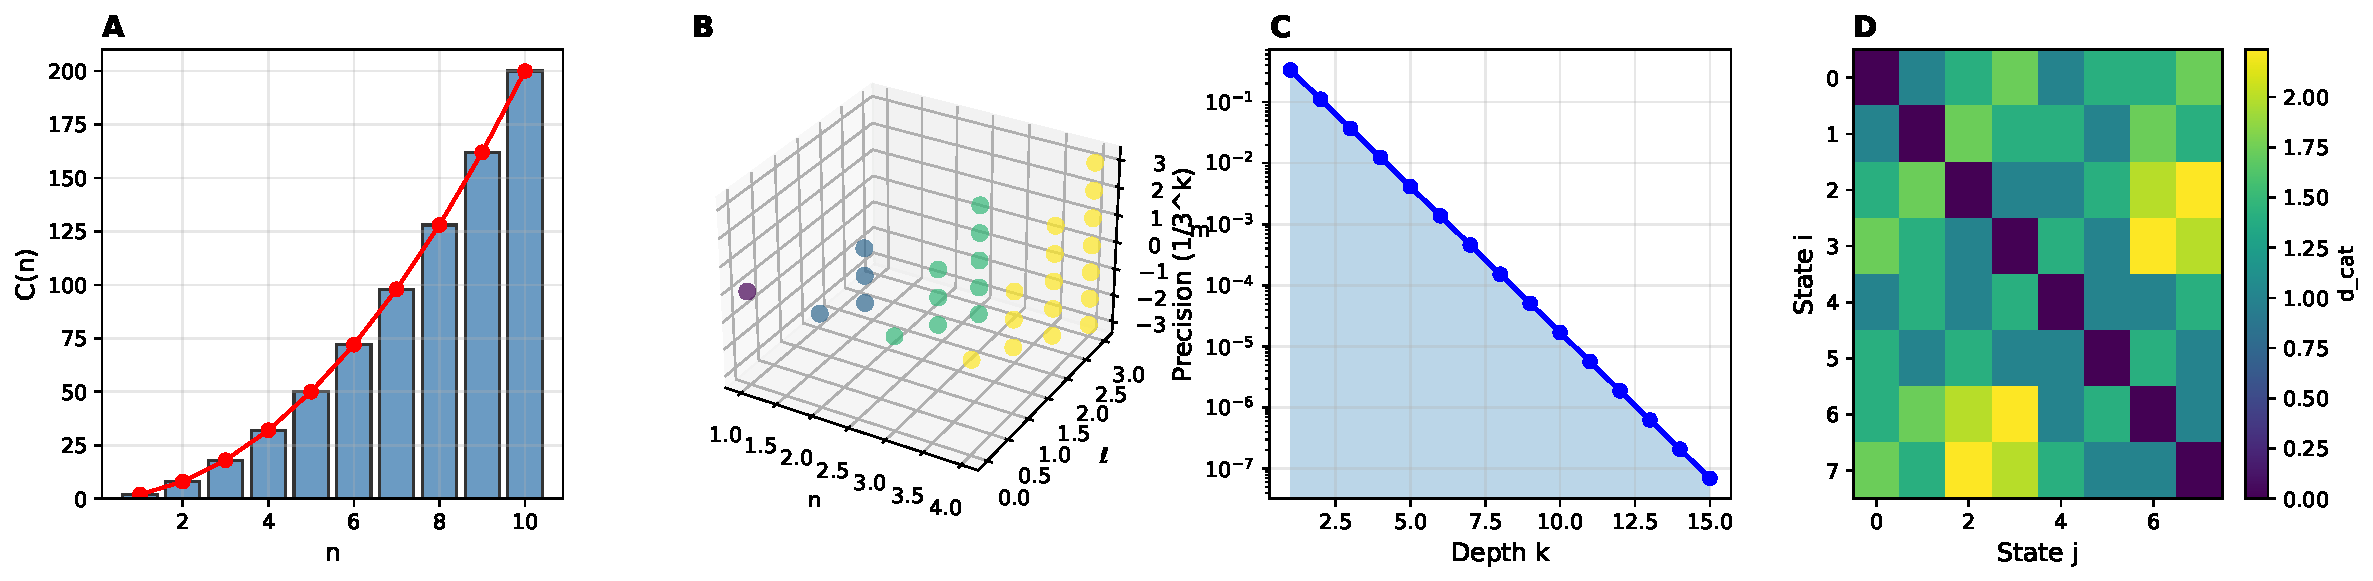
\includegraphics[width=0.9\textwidth]{figures/panel1_partition_geometry.pdf}
\caption{\textbf{Partition Geometry and Categorical Distance.}
\textbf{Panel A (left):} Partition capacity $C(n) = 2n^2$ showing the number of distinguishable categorical states at each depth level $n$. The capacity sequence $(2, 8, 18, 32, 50, \ldots)$ emerges from spherical symmetry constraints in bounded phase space, with red markers indicating computed values matching the analytical quadratic form.
\textbf{Panel B (center-left):} Three-dimensional visualization of partition coordinate space $(n, \ell, m)$ for depths $n \in \{1, 2, 3, 4\}$, with color encoding depth level. Each point represents a valid partition state satisfying the constraint hierarchy $0 \leq \ell \leq n-1$ and $-\ell \leq m \leq \ell$.
\textbf{Panel C (center-right):} Address precision $\epsilon = 3^{-k}$ on logarithmic scale as a function of address depth $k$, demonstrating exponential refinement. At depth $k = 15$, precision reaches $\epsilon \approx 7 \times 10^{-8}$, enabling sub-micron resolution in physical coordinates.
\textbf{Panel D (right):} Categorical distance matrix $d_{\text{cat}}(\sigma_i, \sigma_j)$ for all $C(2) = 8$ states at depth $n = 2$. The Euclidean metric in partition coordinates yields distances independent of spatial separation and optical opacity, enabling opacity-invariant state discrimination.}
\label{fig:partition_geometry}
\end{figure*}

\begin{figure*}[!htbp]
\centering
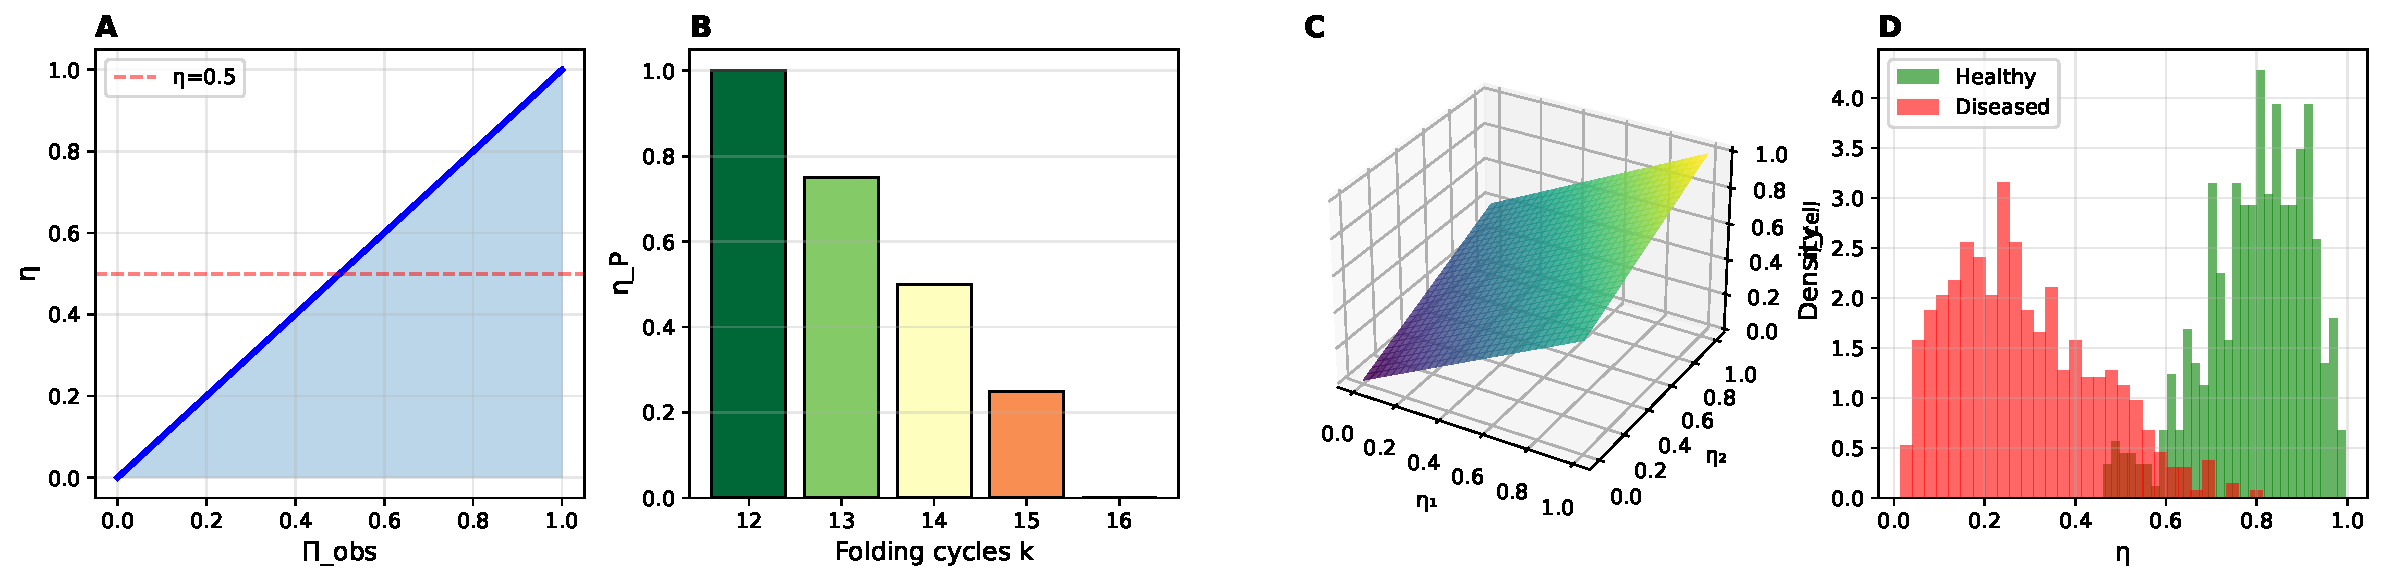
\includegraphics[width=0.9\textwidth]{figures/panel2_coherence.pdf}
\caption{\textbf{Universal Coherence Index and Cellular Coherence.}
\textbf{Panel A (left):} Universal coherence equation $\eta = (\Pi_{\text{obs}} - \Pi_{\text{deg}})/(\Pi_{\text{opt}} - \Pi_{\text{deg}})$ showing linear mapping from observed performance $\Pi_{\text{obs}}$ to coherence index $\eta \in [0,1]$. The horizontal dashed line indicates the critical threshold $\eta = 0.5$ separating functional from dysfunctional states.
\textbf{Panel B (center-left):} Protein folding coherence $\eta_P$ as a function of observed folding cycles $k$, where fewer cycles indicate higher coherence. The color gradient from green ($\eta = 1$, $k = 12$) to red ($\eta = 0$, $k = 16$) visualizes the discrete coherence levels for this oscillator class.
\textbf{Panel C (center-right):} Three-dimensional cellular coherence surface $\eta_{\text{cell}} = w_1\eta_1 + w_2\eta_2$ showing weighted combination of two oscillator coherences with weights $w_1 = 0.6$, $w_2 = 0.4$. The planar surface geometry reflects linear entropic coupling between oscillator classes.
\textbf{Panel D (right):} Coherence distributions comparing healthy (green, $\eta \sim \text{Beta}(8,2)$) and diseased (red, $\eta \sim \text{Beta}(2,5)$) cellular populations. The separation between distributions quantifies diagnostic discriminability using coherence measurements.}
\label{fig:coherence}
\end{figure*}

\begin{figure*}[!htbp]
\centering
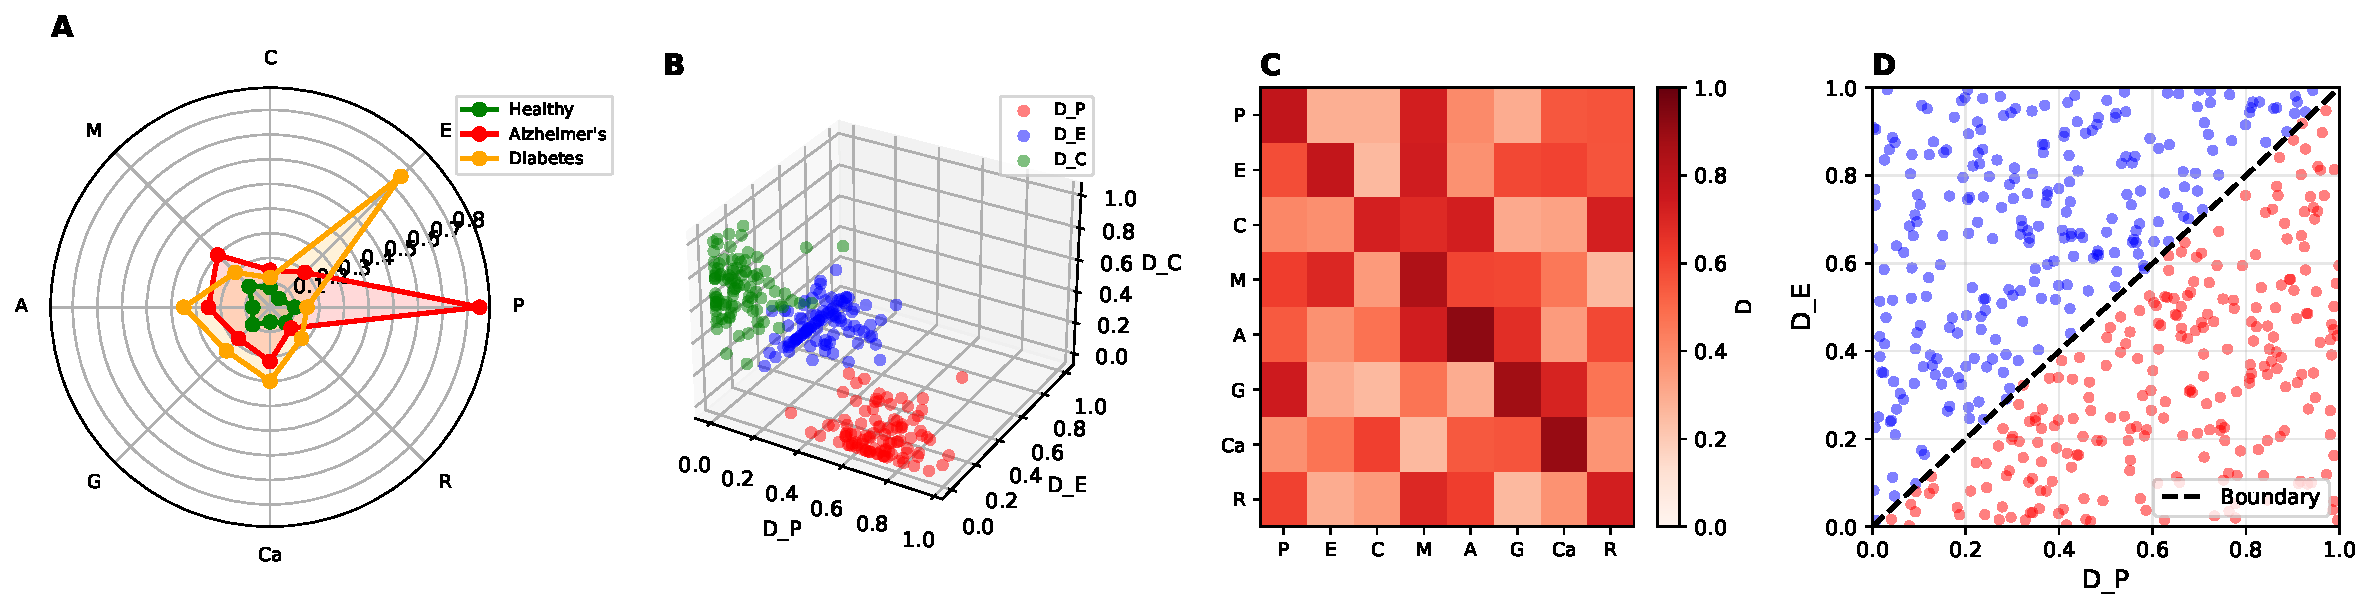
\includegraphics[width=0.9\textwidth]{figures/panel3_disease_state.pdf}
\caption{\textbf{Disease Vector Representation and Classification.}
\textbf{Panel A (left):} Radar chart visualization of disease vectors $\mathbf{D} = (D_P, D_E, D_C, D_M, D_A, D_G, D_{Ca}, D_R)$ across all eight oscillator classes. Healthy state (green) shows uniformly low disease indices, while Alzheimer's (red) exhibits dominant $D_P$ (misfolding) and diabetes (orange) shows dominant $D_E$ (metabolic dysfunction).
\textbf{Panel B (center-left):} Three-dimensional projection of disease space onto $(D_P, D_E, D_C)$ coordinates, showing clustered disease populations. Red, blue, and green clusters represent protein-dominant, enzyme-dominant, and channel-dominant disease classes respectively, demonstrating geometric separability of disease types.
\textbf{Panel C (center-right):} Disease index correlation heatmap across oscillator classes, with diagonal elements representing single-class severity and off-diagonal elements showing cross-class correlations. High diagonal values indicate class-specific disease manifestation patterns.
\textbf{Panel D (right):} Disease classification boundary in the $(D_P, D_E)$ plane, with the diagonal $D_P = D_E$ (black dashed) separating misfolding-dominant (red) from metabolic-dominant (blue) classifications. The geometric criterion $\text{class}(\mathbf{D}) = \arg\max_i D_i$ yields well-defined decision boundaries.}
\label{fig:disease_state}
\end{figure*}

\begin{figure*}[!htbp]
\centering
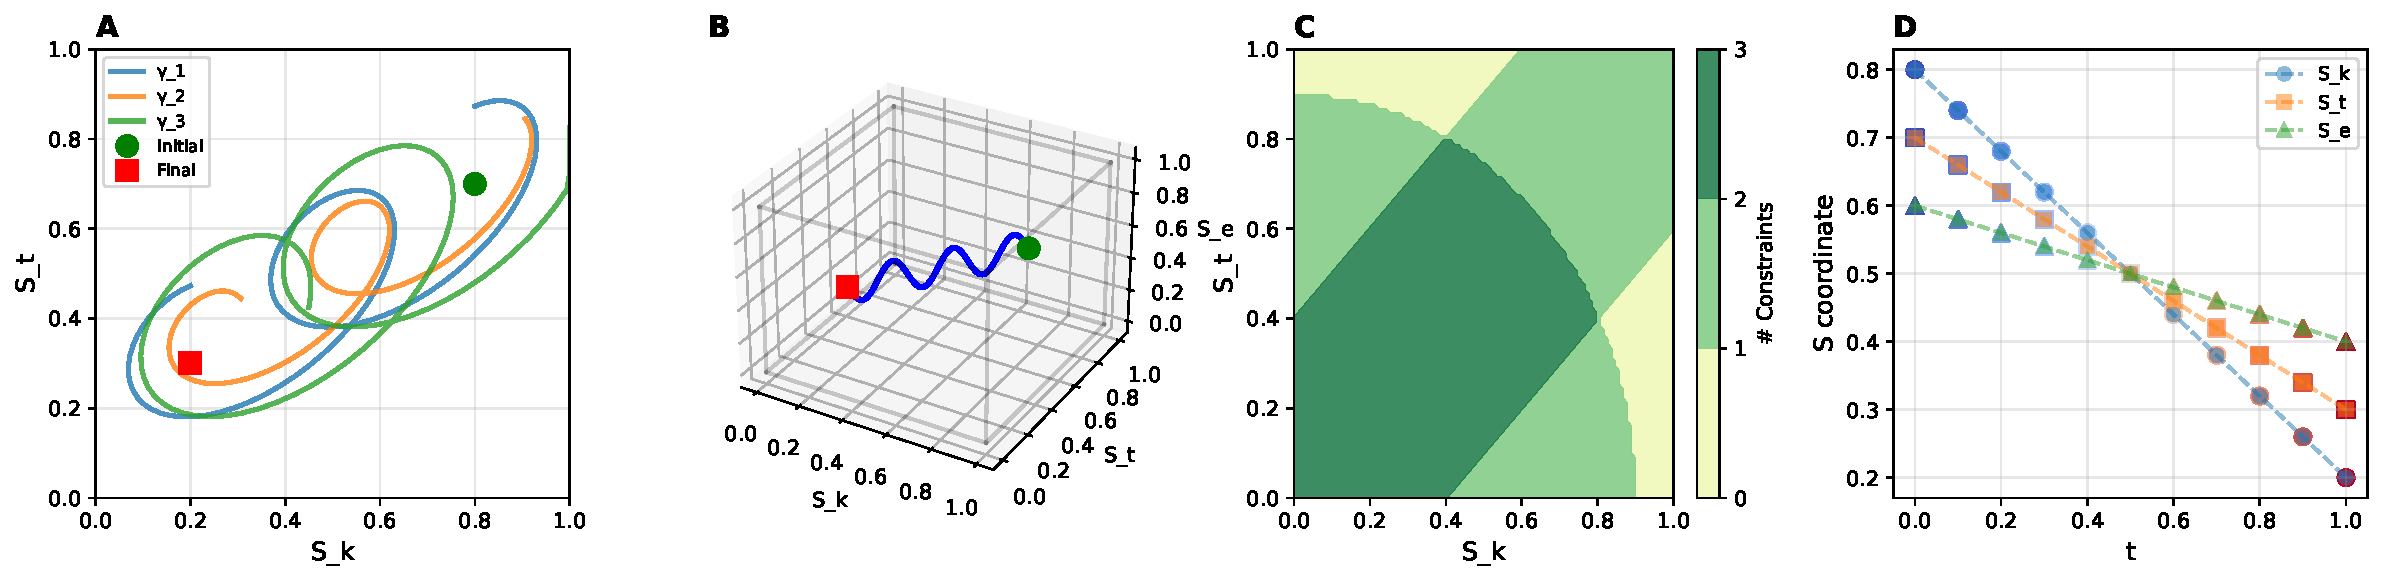
\includegraphics[width=0.9\textwidth]{figures/panel4_trajectory.pdf}
\caption{\textbf{S-Entropy Trajectories and Constraint Satisfaction.}
\textbf{Panel A (left):} Multiple trajectory paths $\gamma_1, \gamma_2, \gamma_3$ in the $(S_k, S_t)$ projection connecting initial state (green circle, high entropy) to final state (red square, low entropy). Different trajectories satisfy different constraint combinations while achieving the same boundary conditions.
\textbf{Panel B (center-left):} Three-dimensional trajectory visualization in the full S-entropy space $(S_k, S_t, S_e)$, with the unit cube edges shown for reference. The trajectory exhibits smooth evolution from high-entropy initial state to low-entropy therapeutic target state.
\textbf{Panel C (center-right):} Constraint satisfaction regions showing the number of simultaneously satisfied constraints (bounded, smooth, energy) at each point in the $(S_k, S_t)$ plane. Darker green indicates more constraints satisfied, identifying the feasible region for valid therapeutic trajectories.
\textbf{Panel D (right):} Trajectory interpolation showing evolution of all three S-entropy coordinates ($S_k$: circles, $S_t$: squares, $S_e$: triangles) as a function of normalized time $t \in [0,1]$. Linear interpolation provides the initial trajectory estimate refined by the COMPLETE algorithm.}
\label{fig:trajectory}
\end{figure*}

\begin{figure*}[!htbp]
\centering
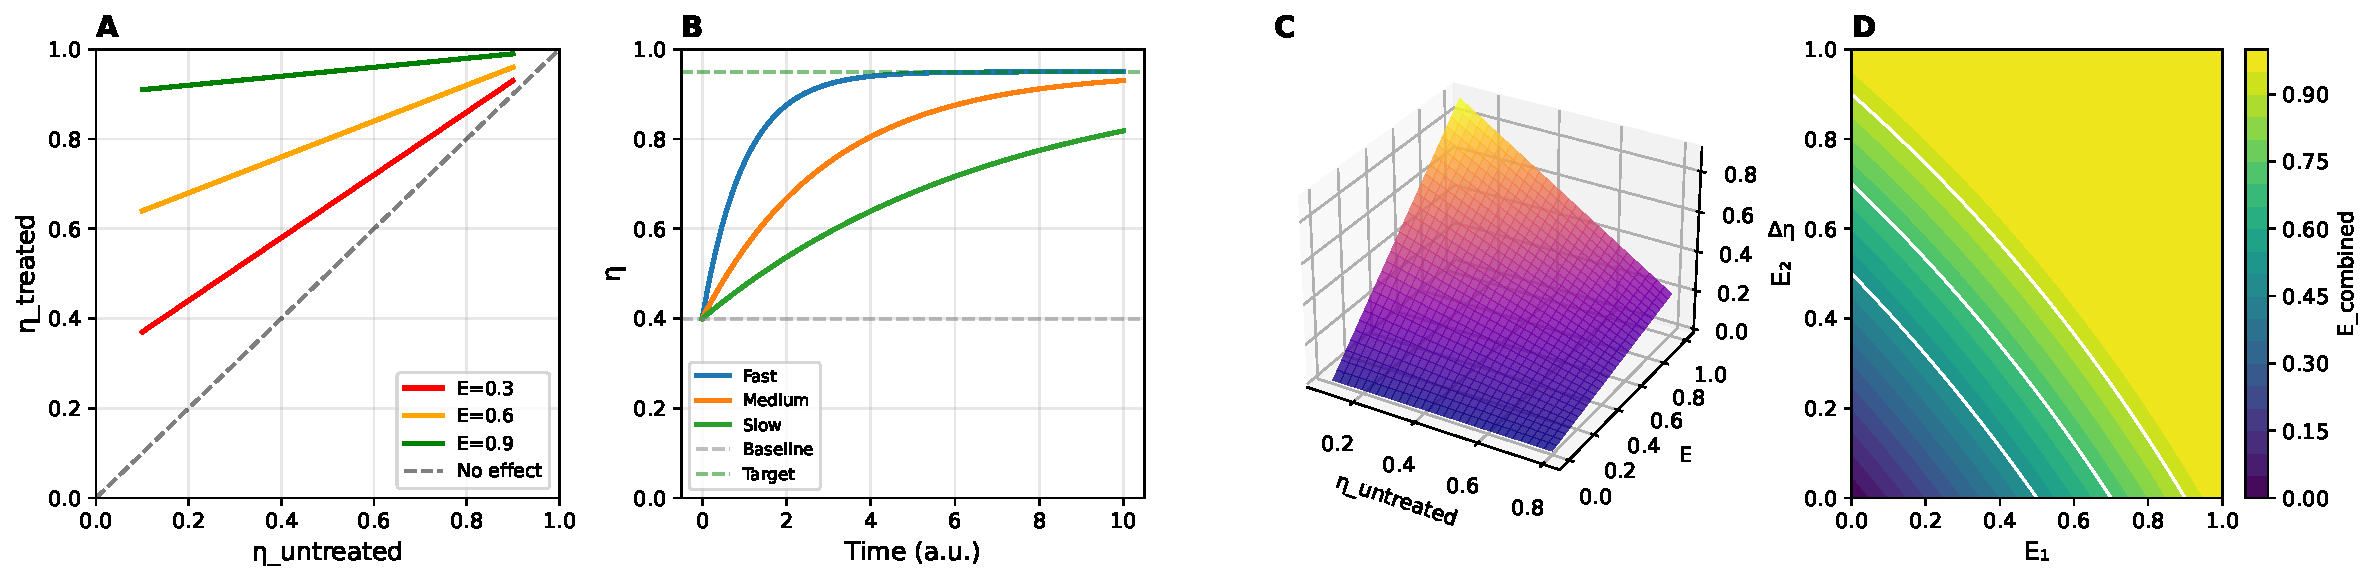
\includegraphics[width=0.9\textwidth]{figures/panel5_therapeutic.pdf}
\caption{\textbf{Therapeutic Efficacy and Treatment Response.}
\textbf{Panel A (left):} Therapeutic efficacy curves showing treated coherence $\eta_{\text{treated}} = \eta_{\text{untreated}} + E(1 - \eta_{\text{untreated}})$ as a function of baseline coherence for efficacies $E \in \{0.3, 0.6, 0.9\}$. Higher efficacy shifts curves toward the target $\eta = 1$, with the identity line (black dashed) representing no treatment effect.
\textbf{Panel B (center-left):} Treatment response trajectories showing coherence recovery $\eta(t) = \eta_0 + (\eta_{\text{target}} - \eta_0)(1 - e^{-t/\tau})$ with time constants $\tau \in \{1, 3, 7\}$ representing fast, medium, and slow responders. Dashed lines indicate baseline ($\eta = 0.4$) and therapeutic target ($\eta = 0.95$).
\textbf{Panel C (center-right):} Three-dimensional efficacy surface showing coherence gain $\Delta\eta = \eta_{\text{treated}} - \eta_{\text{untreated}}$ as a function of baseline coherence $\eta_{\text{untreated}}$ and treatment efficacy $E$. The surface geometry reveals that sicker patients (lower $\eta$) achieve larger absolute improvements at any efficacy level.
\textbf{Panel D (right):} Combination therapy efficacy contours showing combined effect $E_{\text{combined}} = E_1 + E_2 - 0.3E_1E_2$ exhibiting mild synergy. White contour lines at $E = 0.5, 0.7, 0.9$ guide optimal combination selection for target therapeutic outcomes.}
\label{fig:therapeutic}
\end{figure*}
